\documentclass[preprint]{sigplanconf}
\usepackage[utf8]{inputenc}

\usepackage{amsmath}
\usepackage{todonotes}
\presetkeys{todonotes}{inline}{}
\usepackage{graphicx}
\usepackage{tikz}
\usepackage{url}

\begin{document}
\conferenceinfo{FHCP '13}{23 September 2013, Boston, Massachusets, US.} 
\copyrightyear{2013} 
\copyrightdata{[to be supplied]} 

\titlebanner{Preprint, version 1.0}        % These are ignored unless
%\preprintfooter{short description of paper}   % 'preprint' option specified.

\title{A practical survey of functional GPU languages}
%\subtitle{Subtitle Text, if any}

\authorinfo{Martin Dybdal}
           {DIKU, University of Copenhagen}
           {dybber@dybber.dk}
\authorinfo{Philip L. Carlsen}
           {DIKU, University of Copenhagen}
           {plcplc@gmail.com}
\authorinfo{Ken Friis Larsen}
           {DIKU, University of Copenhagen}
           {kflarsen@diku.dk}

\maketitle

\begin{abstract}
  We present a practical survey of a handful of current GPU languages and
  libraries and report on both qualitative and quantitative aspects.

  The survey is practical in the sense that we have taken a few
  algorithms from the domain of computation finance that are used in
  the real world.

  The aim is that the paper can be used to get an overview of the
  current state of existing languages.
\end{abstract}

% \category{CR-number}{subcategory}{third-level}

% \terms
% term1, term2

% \keywords
% keyword1, keyword2

\section{Introduction}
Graphics Processing Units (GPUs) is a cost-efficient choice for
problems with data-parallel solutions. Their massively data-parallel
architecture can deliver a high-throughput for many problems in the
sciences, engineering and finance.

Currently, OpenCL and CUDA are the most popular GPU programming
frameworks in both academia and industry. These two languages are
extension of C and C++ respectively. Both OpenCL and CUDA require
manual memory management, does not provide any means for automatic
deforestation, and offers little abstraction from the underlying
hardware, such that, for example memory coalescing must be on your
mind during implementation.

To make GPU programming more accessible, quite a number of new
high-level data-parallel languages as well as GPU libraries for
existing languages have been developed \cite{Catanzaro2011,
  chakravarty2011accelerating, mainland2010nikola,
  svensson2011obsidian, bergstra2010theano, homepage:rgpu,
  bergstrom2012nested, homepage:bohrium}, though none of them has
achieved the same popularity and attention as programming directly in
OpenCL or CUDA.

In this paper we present our experience of applying a few functional
data-parallel languages to a couple of problems from the domain of
computational finance and report on the current state of GPU
languages. Our scope is both qualitative in terms of the ease with
which algorithms can be formulated and debugged, as well as
quantitative in terms of execution performance.

Our first experiment involves the implementation of a
\emph{quasi-random number generator}, the Sobol sequence generator,
which is an efficient choice for numerical integration and Monte Carlo
simulation \cite{acworth1998comparison}. Our second experiment is the
implementation of an option-pricing algorithm, \emph{the binomial
  method}. Both of these algorithms have been implemented in
Accelerate \cite{chakravarty2011accelerating}, Nikola
\cite{mainland2010nikola}, Copperhead, NESL/GPU and are compared with
efficient CUDA implementations.

%\todo{contributions section?} % 1) Demonstrate lack of composability and
  % abstraction 2) Performance comparison of languages that have not
  % been previously been compared

\section{Subject languages}
\paragraph{NESL/GPU} is a GPU back-end for the parallel functional
programming language NESL \cite{}. The back-end reuses the front-end
of the CPU implementation of NESL, which compiles to an intermediate
language called VCODE, which is a flattened version of the NESL
program. VCODE is then transformed and finally interpreted by issuing
corresponding CUDA kernels.

\paragraph{Copperhead} is a functional DSL for GPU computing embedded
in Python. It is statically typed and uses Hindley-Milner type
inference, even though it is embedded inside a dynamically typed
language. 

* They promise nested data-parallelism, but the current implementation
does not currently support it.

* Nested data-parallelism without flattening

\paragraph{Accelerate} is a parallel functional DSL for array
computations embedded in Haskell. 

 * Clean partition between front-end and back-ends
 * Skeleton-based
 * Hard division between Exp and Acc -> flat data-parallel
 * Single array type, no control over fusion

\paragraph{Nikola} is a parallel functional DSL for array
 computations embedded in Haskell

 * Repa-like interface -> selection of array representation
 * Manual control over fusion
 * Flat data-parallel
 * Only supports map-like higher-order operations (no scan, reduce, etc.)

\section{Case I: Sobol sequence generation}
The first problem that we have used to evaluate the languages is a
quasi-random number generator (QRNG), namely the \emph{Sobol sequence
  generator}. QRNGs is a category of random number generators that
aims at creating samples of low discrepancy, rather than provide good
statistical randomness. QRNGs is thus in contrast with pseudo-random
number generators (PRNGs). A visual comparison of a Sobol-sequence and
a sequence generated by the popular Mersenne Twister PRNG is presented
in Figure~\ref{fig:discrepancyplot}.
\begin{figure}
  \centering
  \begin{minipage}{0.45\linewidth}
    \begin{center}
      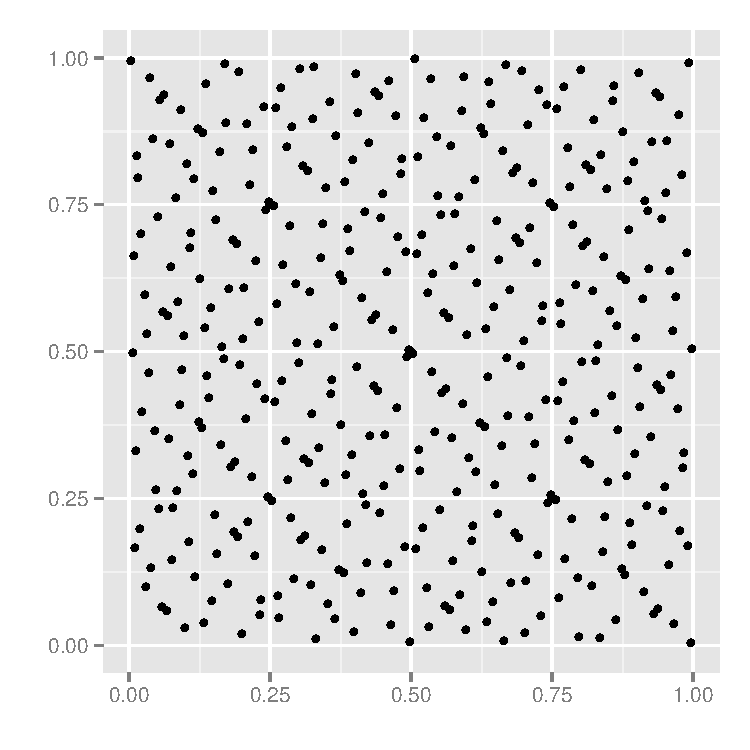
\includegraphics[width=\textwidth]{../report/graphics/2D-sobol-sequence.pdf}

      \hspace{0.55cm}\textbf{(a)}
    \end{center}
  \end{minipage}
  \begin{minipage}{0.45\linewidth}
    \begin{center}
      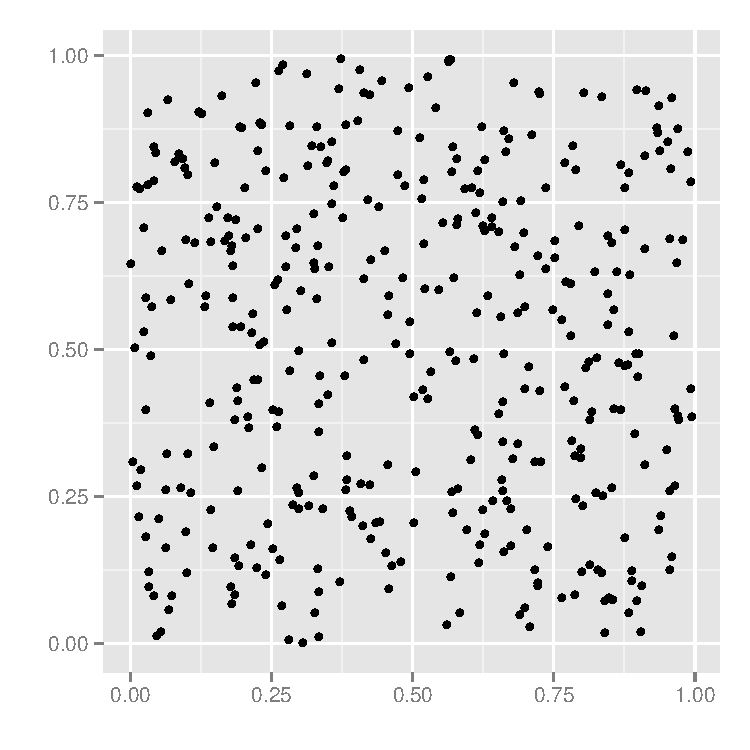
\includegraphics[width=\textwidth]{../report/graphics/2D-mersenne-sequence.pdf}

      \hspace{0.55cm}\textbf{(b)}
    \end{center}
  \end{minipage}

  \caption{\textbf{(a)} A 2D quasi-random sequence from the Sobol
    generator \textbf{(b)} A uniform 2D sequence of pseudo-random
    numbers generated with Mersenne Twister PRNG}
\label{fig:discrepancyplot}
\end{figure}
Figure~\ref{fig:discrepancyplot} illustrates that quasi-random numbers
are generated in a systematic fashion to fill out the sample space
evenly, without clusters nor holes. They are thus a poor choice for
cryptography, but in applications such as numerical integration and
Monte Carlo methods they can be efficient as they can reduce the
number of needed samples. In this case study, we use the Sobol numbers
to perform a simple $\pi$-estimation.

We will first present the implementation of an inductive formulation
of the Sobol algorithm \cite{bratley1988algorithm}, and we will later get
back to a more efficient implementations optimized for GPUs
\cite[Chapter~16]{hwy2011emerald}.

The algorithm is seeded by a so-called \emph{direction vector}. To
generate a Sobol sequence of $32$-bit numbers a direction vector of
length $32$ is required\footnote{Lists of ``good'' direction vectors are
  available online \cite{homepage:sobol:directionvectors}}. Let $v$ be
a direction vector of length $32$, the corresponding Sobol sequence is
then defined by:
\begin{equation}
x_i = v_1i_1 \oplus v_2i_2 \oplus \ldots \oplus v_{32}i_{32}\label{eq:sobol_inductive}
\end{equation}
where $i_j$ is the $j$'th bit in the binary representation of index
$i$. This sequence is then normalised to the $(0,1]$ interval.

It is not hard to translate definition~(\ref{eq:sobol_inductive}) to a
Haskell function working on lists:
\begin{verbatim}
bitVector i = map (fromEnum . testBit i) [0..31]
normalise x = fromIntegral x / 2^32

sobol :: [Int] -> Int -> Float
sobol v i = normalise xi
 where
  xi = foldl xor 0 $ zipWith (*) v (bitVector i)
\end{verbatim}
The \verb|bitVector|-function converts the given index into its binary
representation and \verb|normalise| maps the values to floating-point
numbers in the $(0,1]$ interval.

To generate a complete sequence we can map over all indices:
\begin{verbatim}
sobol1D :: Word32 -> [Word32] -> [Float]
sobol1D m v = map (sobol v) [1..m]
\end{verbatim}
Higher-dimensional sequences can be generated by an additional map:
\begin{verbatim}
sobolND :: Word32 -> [[Word32]] -> [[Float]]
sobolND m vs = map (sobol1D m) vs
\end{verbatim}

Implementing this in NESL is a straight forward translation of the
above Haskell code, which we will not include here. A single piece of
the puzzle was missing though, as NESL does not provide a way to
\emph{fold} using an exclusive-or operation. Instead we had to
implement our own:

\begin{verbatim}
% assumes non-empty argument
function xor_reduce(xs) = xor_scan(xs)[#xs-1] xor xs[#xs-1] $
\end{verbatim}

In the remaining languages, Accelerate, Nikola and Copperhead, the
implementation did not turn out to be as easy, as they do not support
nesting of parallel operations. In Copperhead it should in theory be
possible, but as mentioned previously the current implementation does
not support nesting as promised.

To illustrate we will now show how to implement the inductive
algorithm in Accelerate, which will uncover some problems with the
flat data-parallelism offered by Accelerate, Nikola and Copperhead. We
choose Accelerate for the presentation as it is typed in contrast with
Copperhead and the Array-types are simpler than in Nikola, as they do
not include representation tags.

The type of Accelerate arrays are indexed by their dimensionality,
thus \verb|Array DIM2 Word32| is a two dimensional array (a matrix)
with \verb|Word32| values of regular shape. 
% Accelerate arrays can not be irregular, and the
% two dimensional array will thus be rectangular.

At first, we can translate \verb|sobol| more or less directly:
\begin{verbatim}
normaliseA x = fromIntegral x / 2^bitcount
bitVectorA e = generate (index1 32) gen
 where gen = boolToInt . testBit e . unindex1

sobolA :: Acc (Vector Int) -> Exp Int -> Exp Float
sobolA v i = normalise (the xi)
 where
  xi = fold xor 0 $ zipWith (*) v (bitVector i)
\end{verbatim}

The next step becomes more complicated however, as Accelerate forbids
nested maps. Thus, we cannot write \verb|map sobolA|.  Instead we have
to push this map inside the definition of \verb|sobolA|, a manual
vectorisation of both \verb|bitVectorA| and \verb|sobolA|:
\begin{verbatim}
bitVectors2D :: Exp Int -> Acc (Array DIM2 Int)
bitVectors2D n = generate (index2 n 32) gen
 where gen ix = let Z :. e :. i = unlift ix
                in  boolToInt $ testBit e i
sobol1DA :: Exp Int
         -> Acc (Vector Int)
         -> Acc (Vector Float)
sobol1DA m vec = map normalise xi
 where
  xi = fold xor 0 $ zipWith (*) vecRep mat
  mat = bitVectors2D m
  vecRep = replicate (lift (Z :. m :. All)) vec
\end{verbatim}
What we have done is to vectorise every operation used in
\verb|sobolA|, such that they operate on values of an additional
dimension.

If we wish to generate $n$-dimensional Sobol sequences, we will again
face the same barrier and we have to do a vectorisation in the
direction vector argument of \verb|sobol1DA|. Where we use
two-dimensional arrays we have to use three-dimensional arrays. We
will not present a \verb|sobolNDA|, but just mention that in all
parts of the sobol1DA above we would have to take the additional
dimension into account.

% \begin{verbatim}
% sobolNDA :: Acc (Array DIM2 Word32) -> Exp Int -> Acc (Array DIM2 Float)
% sobolNDA dirvs n = map normalise $ fold xor 0 $ zipWith (*) dirvs_rep (bitVectors n j)
%   where
%     j = fst . unindex2 . shape $ dirvs
%     dirvs_rep = replicate (lift $ Z :. n :. All :. All) dirvs
%     normalise x = fromIntegral x / 2^bitcount
%     bitVectors n j = generate (lift $ Z :. n :. j :. constant bitcount) helper
%       where
%         helper ix = let Z :. e :. _ :. i = unlift ix :: Z :. Exp Int :. Exp Int :. Exp Int
%                     in fromIntegral . boolToInt $ testBit e i
% \end{verbatim}

This example is a small scale illustration of a problem in languages
that disallow nested array operations. That is, flat data-parallel
languages. The fact that we could not apply \verb|sobolA| in the
context that we wanted, but had to change its inner workings showcases
a lack of composability and abstraction in such languages.

In a larger setting, the mapped function could be arbitrarily complex,
thus making the vectorisation hard to do by hand, or the function could
reside in an external library, making the transformation impossible.

Computing $\pi$ has not been covered in the above section,
and the computation is straight forward in all languages except
Nikola. To compute $\pi$ from the 2-dimensional Sobol-sequence we need
a reduction operation, which is not included in Nikola. Nikola does
only provide a few mapping operations and a iteration construct for
sequential iteration inside a CUDA-kernel. Instead we have to use a
divide-and-conquer algorithm which requires the scheduling of
$O(lg~n)$ kernels or reduce on the CPU.

% \paragraph{Thrust} \todo{Perhaps some note on why I selected to use a
%   combination of raw CUDA and Thrust?}

\subsection{Alternative algorithm}
The inductive algorithm presented above requires a linear amount of
exclusive-or operations in the bit representation used. An alternative
recursive algorithm have been shown that uses a single exclusive-or
operation for each number. This recursive algorithm have been
optimized for GPUs by Thomas Bradley et
al. \cite[Chapter~16]{hwy2011emerald}. An implementation of this
GPU-optimized algorithm is included as an example in the CUDA SDK. The
algorithm progresses by first filling a block of values using the
inductive algorithm and then fill each subsequent block from a
recursive formulation using the values from the preceding iteration.

In neither Accelerate, Nikola or Copperhead can we implement this
GPU-optimized algorithm, as they lack a construct for iterative array
construction. Such a construct is commonly known as \texttt{unfold}
and would in Accelerate have a type similar to:

\todo{Does NESL have such an operation?}

\begin{verbatim}
unfold :: Elt a => Exp Int -> (Exp Int -> a -> a)
       -> Array sh a -> Array (sh :. Int) a
\end{verbatim}

Where the first argument defines the number of times to unfold, and
the block size is defined from the size of the array argument.

\subsection{Benchmark}
\emph{TODO present benchmark of calculating $\pi$ using Sobol-sequences}

\emph{TODO evaluate benchmark results. Mention that both Nikola and
  Accelerate code is fused into a single kernel. CUDA uses several
  kernels, because no automatic fusion is performed}

\section{Case II: Binomial option pricing}
In this section we look at the problem of \emph{option pricing}. The
name \emph{option} is used collectively for a range of different
financial contracts which are time-limited opportunities to buy or
sell some underlying asset, for instance a stock. In the contract a
specific \emph{strike price} is also given, which is the pre-agreed
amount of money for buying or selling.

A particular type of options, \emph{American style options}, are
characterised by having a pre-determined constant strike price $K$,
and may be exercised in a time-interval up until the expiration time
$T$. A \emph{call option} on asset $A$ grants the right to buy $A$,
whereas a \emph{put option} grants the right to sell.

\begin{verbatim}
data OptType = Call | Put
data Option = Option
 { opttyp :: OptType -- Call or Put option?
 , s0     :: Float   -- Current price of underlying
 , strike :: Float   -- Strike price
 , expiry :: Int     -- Expiry in years
 , r      :: Float   -- Riskless rate
 , vol    :: Float   -- Volatility
 }
\end{verbatim}

To estimate the price of an American option we have to simulate the
price development of the underlying, as there is no known closed-form
analytic solution. For the simpler case of \emph{European style
  option} pricing, a closed-form solution is available in the
Black-Scholes formula \cite{black1973pricing}.

A relatively simple discrete time model for computing the price of an
American style option is the \emph{standard binomial
  model}~\cite{cox1979option}.  The basic assumption is that the price
of the underlying follows a binomial process over equally spaced time
steps. This makes it possible to write out the possible future states
of the underlying. Moving a single time step forward, the binomial
process produces two possible future states of the underlying. The
value of the underlying can go either up or down with probabilities
$q$ and $(1 - q)$ respectively. We denote the rate of up and down
movement as $u$ and $d$ respectively. The change over one period
$\Delta t$ is thus given as:

\begin{equation}
S(t+\Delta t) = \left\{
  \begin{array}{ll}
    S(t)u & \quad \textrm{with probability $q$} \\
    S(t)d & \quad \textrm{with probability $1-q$}
  \end{array} \right.
\end{equation}

Iterating this procedure starting at time $t_0$ (now), where the
current price of the underlying is known to be $S(t_0)$, we will
obtain a binomial tree as the one in
Figure~\ref{fig:binomial-tree}. In this case we have used three
periods, the expiration time $T$ is $t_3$, and we have assumed that
$u\cdot d = 1$.

\begin{figure}
  \centering
  \tikzstyle{nodestyle} = [text centered, minimum size=0.42cm, inner sep=0]

\begin{tikzpicture}
  \node at (0,0) [nodestyle] (S1) {$S(t_0)$};

  \node at (-1, -1) [nodestyle] (dS) {$dS(t_0)$};
  \node at ( 1, -1) [nodestyle] (uS) {$uS(t_0)$};

  \node at ( 2, -2) [nodestyle] (u2S) {$u^2S(t_0)$};
  \node at ( 0, -2) [nodestyle] (S2) {$S(t_0)$};
  \node at (-2, -2) [nodestyle] (d2S) {$d^2S(t_0)$};

  \node at ( 3, -3) [nodestyle] (u3S) {$u^3S(t_0)$};
  \node at ( 1, -3) [nodestyle] (uS2) {$uS(t_0)$};
  \node at (-1, -3) [nodestyle] (dS2) {$dS(t_0)$};
  \node at (-3, -3) [nodestyle] (d3S) {$d^3S(t_0)$};

  \node at (-4.5,  0) [] (t0) {$S(t_0) =$};
  \node at (-4.5, -1) [] (t0) {$S(t_1) =$};
  \node at (-4.5, -2) [] (t0) {$S(t_2) =$};
  \node at (-4.5, -3) [] (t0) {$S(t_3) =$};

  \path[-latex]
     (S1) edge (uS)
     (S1) edge (dS)

     (uS) edge (S2)
     (dS) edge (S2)
     (uS) edge (u2S)
     (dS) edge (d2S)

     (u2S) edge (u3S)
     (u2S) edge (uS2)
     (S2)  edge (uS2)
     (S2)  edge (dS2)
     (d2S) edge (dS2)
     (d2S) edge (d3S);
\end{tikzpicture}

\vspace{2mm}

\caption{Lattice generated by the binomial process of a single
  underlying over three periods ($T=t_3$). The root node represents
  the current price of the underlying and the leafs represents
  possible values at expiration time.}
\label{fig:binomial-tree}
\end{figure}

We represent the model parameters as:
\begin{verbatim}
data BinParams = BinParams 
  { u :: Float
  , d :: Float
  , q :: Float
  }
\end{verbatim}

The leaf nodes represents the possible values of the underlying at
the expiration time. After $n$ time steps, we will have $n+1$ leafs, which
values we can compute by:
\begin{verbatim}
leafs p s0 n = [s0 * exp(vsdt * fromIntegral (2*i-n))
        | i <- [0..n :: Int]]
\end{verbatim}
These leafs represents all the possible prices at expiration time, and
for each possibility we can determine whether it would worthwhile to
exercise our option right. Depending on whether we are pricing a
\emph{put} or a \emph{call} option, the option values at expiration
will be either of:
\begin{verbatim}
finalPut  p (AOpt{..}) = map (\v -> max (strike - v) 0) $ leafs p s0 n
finalCall p (AOpt{..}) = map (\v -> max (v - strike) 0) $ leafs p s0 n
\end{verbatim}
From this point, we can discount backward one time-step at a time to
calculate the option price at time zero, while taking into account the
probabilities $q$ and $1-q$.
\begin{verbatim}
stepbackward p opt prev i =
    zipWith3 (\up down st -> max (strike - st) 
                                 (e^(-r*dt) * (q*up + (1-q)*down)))
             prev
             (tail prev)
             (leafs i)
\end{verbatim}
Everything can then be combined:
\begin{verbatim}
binomial p opt@(AOpt{..}) =
    head $ foldl (stepbackward p opt) (finalPut opt) [n, n-1 .. 1]
\end{verbatim}

In our benchmarks we will price European style options, such that we
can use Black Scholes to evaluate the correctness of our
implementation. The performance characteristics should map directly to
that of American option pricing.

We now implement this pricing algorithm as a parallel program in
Accelerate. We cannot parallelize the outer \verb|foldl| operation,
because of the dependencies between each iteration. Thus, the
parallelisation of \verb|binomial| must be found in the calls to
\verb|map| and \verb|zipWith3|. Thus our implementation use an
ordinary Haskell fold running on the CPU and each call to
\verb|stepbackward| will be executed on the GPU.
\begin{verbatim}
Accelerate implementation of binomial pricer
\end{verbatim}

We have the same problem with dependencies between iteration when
writing the program in CUDA, if we want to use all the scalar
processors. Becase CUDA does not provide a way to synchronize between
work-groups other than adding a synchronization barrier between
individual kernel calls.

In Figure \emph{TODO} we present the actual execution times.

An alternative parallelisation strategy is to price several
options simultaneously, a portfolio pricer. Thus, we investigate
the parallelisation opportunities for:
\begin{verbatim}
binomialPortfolio options = map binomial options
\end{verbatim}

An efficient implementation can be found in the CUDA SDK, and this is
the implementation we want to compare against. In the algorithm
present there, ...

\begin{itemize}
% \item Introduce binomial option pricing
% \item Show how that would lead to host synchronisation in each iteration
% \item See if we can find some paper about the overhead incurred by
%   extraneous kernel launches
% \item Say that an alternative parallelisation scheme prices several
%   options simultaneously: portfolio pricing.
\item Show that we have a hard time expressing such a portfolio
  pricer, because of irregularity when performing the manual
  vectorisation
\item Present a benchmark showing the benefit of having portfolio
  pricer rather than pricing each option in their own kernels
  sequentially.
\end{itemize}

\section{Qualitative language comparison}
\todo{Section with remarks about level of maintenance/developer
  activity, quality of compiler e.g. error messages, and how often you
  encounter problems (e.g. CUDA unspecified launch failure). See list
  on Google Drive, number of users}

\section{Related work}
Disposition:
\begin{itemize}
\item Mention some of the languages we haven't tested. See if can put
  them in categories where the above problems are present and aren't,
  even though we haven't tested them as much.
\end{itemize}

\section{Future work}
Disposition;
\begin{itemize}
\item Extend the survey to cover additional languages:
  Modern GPU, Bohrium, Theano, CUB
\item Extend the survey to cover additional problems:
  LSM, 7 dwarfs
\item Create a larger performance benchmark of the different
  languages
\item Comparison of GPU-NESL VCODE and Bohrium bytecode
can Bohrium be used as a NESL backend?
\end{itemize}

\section{Conclusion}
Summarise, mention GPU-NESL and other languages we haven't tested.

\acks

Acknowledgments, if needed.


\bibliographystyle{abbrvnat}
\bibliography{../bibliography/bibliography}

\end{document}

% LocalWords:  OpenCL CUDA GPU Carlsen Dybdal Sobol Nikola QRNG QRNGs
% LocalWords:  PRNGs Mersenne PRNG dimensionality composability
% LocalWords:  vectorisation Scholes
